\chapter{Samples Preparation}\label{ch:samples}
This chapter describes the data and Monte Carlo samples used for the cross section analyses, % as well as the work necessary to prepare the samples in a usable state for the physics analyses.
\section{LArIAT Data}
\section{LArIAT Monte Carlo}
\subsection{G4Beamline}\label{beamlineComposition}
\subsection{Data Driven MC}\label{sec:DDMC}


\section{Energy Calibration}\label{ch:EnCalibration}
\section{Tracking Studies}
In this section, we describe three studies. The first is a justification of the selection criteria for the beamline handshake with the TPC information.  We perform this study to boost  the correct identification of the particles in the TPC associated with the beamline information, while maintaining sufficient statistics for the cross section measurement. 
The second study is an optimization of the tracking algorithm, with the scope of maximizing the identification of the hadronic interaction point inside the TPC. These two studies are related, since the optimization of the tracking is performed on TPC tracks which have been matched to the wire chamber track; in turn, the tracking algorithm for TPC tracks determine the number of reconstructed tracks in each event used to try the matching with the wire chamber track. Starting with a sensible tracking reconstruction, we perform the WC2TPC matching optimization first, then the tracking optimization. The WC2TPC match purity and efficiency  are then calculated again with the optimized tracking.


%\section{MC sample and WC2TPC match}
We perform the following studies on a MC sample of 191000 kaons and 359000 pions produced with the DDMC technique. DDMC particles are shot from the WC4 location into the TPC following the beam profile.
We mimic the matching between the WC and the TPC track on Monte Carlo by constructing a fake WC track using truth information at wire chamber four. We then apply the same WC to TPC matching algorithm as in data described in \ref{ch:WC2TPCMatchMethod}. 



%In data, we attempt to uniquely match one WC-Track to one and only one reconstructed TPC track. This match is done by using in the $X$ and $Y$ coordinate of the extrapolated WC-Track to the upstream most point of the reconstructed TPC Track and by using the angle between the incoming track angle and the reconstructed TPC. We define $\Delta$X as the difference between the $x$ position of the most upstream point of the TPC track and the $x$ position of the WC track as projected to the TPC front face. $\Delta$Y is defined analogously. We define  $\Delta$R as $ \Delta \text{R} =  \sqrt{ \Delta \text{X}^2 +  \Delta \text{Y}^2}  $. The angle between the incident WC Track and the TPC track in the plane that contains them defines $\alpha$.  

%We define a match between WC-track and TPC reconstructed track if  $\Delta \text{R} < r_{T}$, $\alpha < \alpha_{T}$ and the Z position of the first reconstructed point of the TPC track is within 2 cm from the TPC front face. The determination of the best $r_{T}$ and $\alpha_{T}$ is the scope of the following section.

%In MC, we mimic the matching between the WC and the TPC track on Monte Carlo by constructing a fake WC track using truth information at wire chamber four. We then apply the same WC to TPC matching algorithm as in data. 

\subsection{Selection Study for the Wire Chamber to TPC Match}\label{ch:WC2TPCMatchOptimization}
Plots I want in this section:
\begin{enumerate}
\item WC2TPC MC DeltaX, DeltaY and $\alpha$
\end{enumerate}


Scope of this study is assessing the goodness of the wire chamber to TPC match on Monte Carlo and decide the selection values we will use on data. A word of caution is necessary here. With this study, we want to minimize pathologies associated with the presence of the primary hadron itself, e.g. the incorrect association between the beamline hadron and its decay products inside the TPC.  Assessing the contamination from pile-up\footnote{We remind the reader that the DDMC is a single particle Monte Carlo, where the beam pile up is not simulated.}, albeit related, is beyond the scope of this study.

In MC, we are able to define a correct WC2TPC match using the Geant4 truth information. We are thus able to count how many times the WC tracks is associated with the wrong TPC reconstructed track. 

We define a correct match if the all following conditions are met:
\begin{itemize}
\item[-] the length of the true primary Geant4 track in the TPC is greater than 2 cm,  
\item[-] the length of the reconstructed track length is greater than 2 cm,
\item[-] the Z position of the first reconstructed point is within 2 cm from the TPC front face
\item[-] the distance between the reconstructed track and the true entering point is the minimum compared with all the other reconstructed tracks.
\end{itemize}

In order to count the wrong matches, we consider all the reconstructed tracks whose Z position of the first reconstructed point lies within 2 cm from the TPC front face. Events with true length in TPC $<$ 2 cm are included. 
Since hadrons are shot 100 cm upstream from the TPC front face, the following two scenarios are possible from a truth standpoint: 
\begin{itemize}
\item[[$Ta$]] the primary hadron decays or interact strongly before getting to the TPC,
\item[[$Tb$]] the primary hadron enters the TPC.
\end{itemize}

Once we choose the selection cuts to determine a reconstructed wire chamber-to-TPC match $r_{T}$ and $\alpha_{T}$, the following five scenarios are possible in the truth to reconstruction interplay : 
\begin{itemize}
\item[1)] only the correct track is matched
\item[2)] only one wrong track is matched 
\item[3)] the correct track and one (or more) wrong tracks are matched
\item[4)] multiple wrong tracks  matched.
\item[5)] no reconstructed tracks are matched
\end{itemize}

Since we keep only events with one and only one match, we discard cases 3), 4) and 5) from the events used in the cross section measurement. For each set of $r_{T}$ and $\alpha_{T}$ selection value, we define purity and efficiency of the selection as follows:
\begin{equation}
\text{Efficiency} = \frac{\text{Number of events correctly matched}}{\text{ Number of events with primary in TPC}}
\end{equation}

\begin{equation}
\text{Purity} = \frac{\text{Number of events correctly matched}}{\text{Total number of matched events}}.
\end{equation}

Figure \ref{fig:EffPurityK} shows the efficiency (left) and purity (right) for wire chamber-to-TPC match as a function of the radius, $r_{T}$, and angle, $\alpha_{T}$, selection value. It is apparent how both efficiency and purity are fairly flat as a function of the radius selection value at a given angle. This is not surprising. Since we are studying a single particle gun Monte Carlo sample, the wrong matches can occur only for mis-tracking of the primary or for association with decay products;  decay products will tend to be produced at large angles compared to the primary, but could be fairly close to the in $x$ and $y$ projection of the primary. The radius cut would play a key role in removing pile up events. 

For LArIAT cross section measurements, we generally prefer purity over efficiency, since a sample of particles of a pure species will lead to a better measurement. Obviously, purity should be balanced with a sensible efficiency to avoid rejecting the whole sample. 

We choose $(\alpha_{T}$, $r_{T}) = (8 \text{ deg}, 4 \text{ cm} )$ and get a MC 85\% efficiency and 98\% purity for the kaon sample and a MC \textcolor{red}{BOH}\% efficiency and 98\% purity for the \textcolor{red}{BOH} sample.


\begin{figure}[hpbt]
\centering
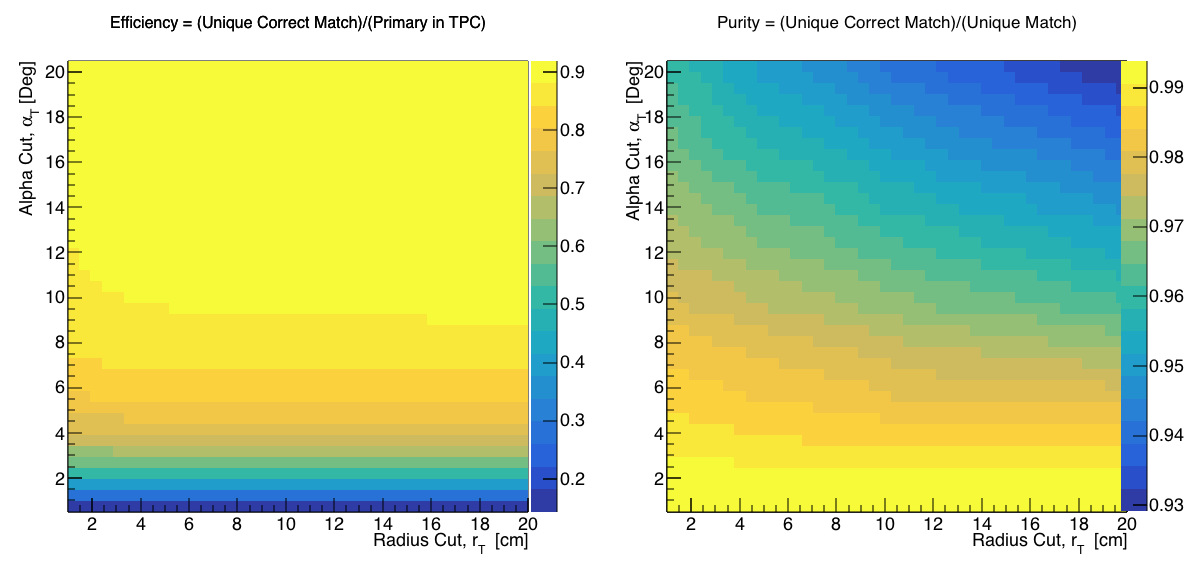
\includegraphics[width=15cm]{Chapter-5/Images/KEffPurity.png}
\caption{Efficiency (left) and purity (right) for wire chamber-to-TPC match as a function of the radius and angle selections.}
\label{fig:EffPurityK}
\end{figure}

\subsection{Interaction Point Optimization}\label{ch:TrackingOptimization}
Scheme of this subsection
\subsubsection{Brief Explanation of the reconstruction chain}
\subsubsection{Explanation of clustering parameters}
\subsubsection{Figure of merit and  spanning of cluster}
\subsubsection{Important numbers out of this optimization}


Plots I want in this section:
\begin{enumerate}
\item Delta L, reco - true
\item Delta L, reco - true Elastic, Delta L, reco - true Inelastic, other
\item Length Quality cut
\item Efficiency as a function of true KE and Angle
\end{enumerate}


\subsection{Tracking spatial and angular resolution}
Scope of this study is understanding and comparing the tracking spatial and angular resolution on data and MC.
We start by selecting all the WC2TPC matched tracks. 
We fit a line on all the space points of the track and calculate the $\chi^2$. The $\chi^2$ distribution for data and MC is shown in Figure \ref{fig:Chi2AllPts}.

For the spatial and angular resolution study, we reject tracks with less than 14 space points. For each track, we order the space points according to their Z position and we split them in two sets: the first set counts all the points belonging to the first half of the track and the second set counts all the points belonging to the second half of the track. We remove the last 5 points in the first set and the first 5 points in the second set, so to have a gap in the middle of the original track. We fit the first and the second set of points with a line separately. We reject the event entirely if the  $\chi^2$ for the fit of either of the halves is greater than four.  We define a track middle plane as the plane perpendicular to the original track fit, positioned in the middle of its length. We project the tracks on the middle plane and calculate the impact parameter, $d$, i.e. the distance between the projected points. We also calculate the angle between the original track direction and the fit of the first and second half, called $\alpha_1$ and $\alpha_2$ respectively. The spatial resolution of the track will be $\sigma_S = \frac{d}{\sqrt 2}$ while the angular resolution of the tracks will be  $\sigma_\alpha = \alpha_1 - \alpha_2$. The distributions for data and MC for $\sigma_\alpha$ and $\sigma_S$ are given in \ref{fig:trackingResolution}.


\subsection{Estimate of $E_{loss}$ before the TPC}
The beamline particles travel a path from when their momentum is measured by the beamline detector, until they are tracked inside the TPC. In the current LArIAT geometry, a particle leaving the fourth wire chamber will encounter the materials listed in Table \ref{tab:budget} before being registered again. The energy lost by the particle in this non instrumented material modifies the particle's kinetic energy and directly affects the cross section measurement, as shown in equation \ref{eq:enFF}.

\begin{table}[h!]
\centering
\begin{tabular}{|l|l|l|}
\hline
Material  & density {[}g/cm$^3${]} & width {[}cm{]}    \\ \hline
Fiberglass laminate (G10)      & 1.7                             & 1.28                              \\
Liquid Argon                           & 1.4                             & 3.72                             \\
Stainless Steel                        & 7.7                            & 0.23                             \\
Titanium                                  & 4.5                            & 0.04                             \\ 
Air                                            &  1.2 $\cdot10^{-3}$  & 89.43                              \\
Plastic Scintillator                    & 1.03                          & 5.30                              \\ \hline
\end{tabular}
\caption{LArIAT material budget from WC4 to the TPC Front Face.}
\label{tab:budget}
\end{table}


We estimate the uncertainty on the energy loss between the beamline momentum measurement and the TPC, $E_{loss}$, using the DDMC pion sample. We shoot pions from WC4 with the same momentum distribution as in the beamline data and plot the true $E_{loss}$ for that sample. The distribution for $E_{loss}$ for the pion sample is shown in Figure \ref{fig:Eloss}. We estimate the energy loss for pions to be $E_{loss} = 37 \pm 7 $~MeV where we use the average energy lost as the central value and the standard deviation of the distribution as the uncertainty. 

\begin{figure}[hpbt]
\centering
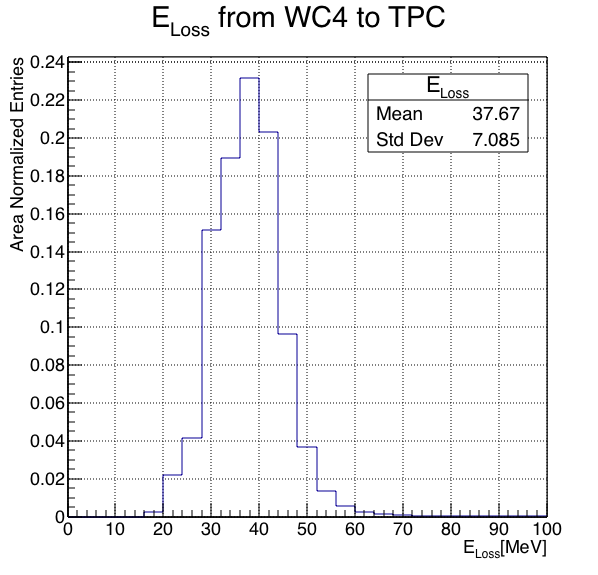
\includegraphics[scale=0.4]{Chapter-5/Images/cELossPions.png}
\caption{Energy loss by simulated negative pions downstream from WC4 and upstream from the TPC.}
\label{fig:Eloss}
\end{figure}






